\providecommand\lcode{\begingroup \small\urlstyle{tt}\Url}
\providecommand\lident{\begingroup \small\urlstyle{tt}\Url}

\chapter{Propagating Information using SSA\Author{F. Brandner, D. Novillo}}

\newcommand{\obacht}[2]{\marginpar{\tiny\textbf{#1:} #2}}

\graphicspath{{img/}{constant_propagation_is_easier/img/}{part3/constant_propagation_is_easier/img/}}

\lstdefinelanguage{DNlisting}
{
  morekeywords={PHI,ASSERT_EXPR},
  morekeywords=[2]{struct,const,int,void,for,if,throw,call,return},
  sensitive=true,
%   morecomment=[s]{<!--}{-->},
%   morestring=[b]",
}

\lstset{
  mathescape=true,
  language=DNlisting,
  basicstyle=\small,
  keywordstyle=\ttfamily,
  keywordstyle=[2]\bfseries,
%   identifierstyle=,
%   stringstyle=\color{black}\ttfamily,
%   commentstyle=\it,
%   moredelim=[is][\color{MyDarkGreen}\ttfamily]{|}{|}
  numbers=left
}

\section{Overview}

A central task of compilers is to \emph{optimize} a given input program such
that the resulting code is more efficient in terms of execution time, code size,
or some other metric of interest. However, in order to perform optimizations and
program transformations typically some form of \emph{program analysis} is
required in order to determine if a given transformation is applicable, to
estimate its profitability, or guarantee correctness.

\emph{Data flow analysis}~\cite{novillo:bib:NNH99} is a simple, yet powerful,
approach to program analysis that is utilized by many compiler frameworks and
program analysis tools today. We will introduce the basic concepts of
traditional data flow analysis in this chapter and show that \emph{static single
assignment} form (SSA) facilitates the design and implementation of equivalent
analyses, while leveraging properties of programs in SSA form allows to reduce
the compilation time and memory consumption.

Traditionally, data flow analysis is performed on a \emph{control flow graph}
(CFG) representation of the input program, where nodes in the graph represent
operations and edges the possible flow of program execution.
Information on certain \emph{program properties} is propagated among
the nodes along the control flow edges until the computed information at the
nodes stabilizes, i.e., no \emph{new} information can be devised from the
program.

The \emph{propagation engine} presented in the following sections is an
extension of the well known approach by Wegman and Zadeck for \emph{sparse
conditional constant propagation}~\cite{bib:wegman.ea-91} (also known as
SSA-CCP). Instead of using the CFG they represent the input program as an
\emph{SSA graph}~\cite{novillo:bib:CFRWZ91}. Operations are again represented as
nodes in this graph, however, the edges represent \emph{data dependencies}
instead of control flow. This representation allows a selective propagation of
program properties among data dependent graph nodes only. As before, the
processing stops when the information at the graph's nodes stabilizes. The basic
algorithm is not limited to constant propagation and can also be applied to
efficiently solve a large class of other data flow
problems~\cite{novillo:bib:N05} as will be shown in the following.

The remainder of this chapter is organized as follows. First, the basic concepts
of (traditional) data flow analysis are presented in
Section~\ref{novillo:sec:preliminaries}. This will provide the theoretical
foundation and background for the discussion of the SSA-based propagation
engine in Section~\ref{novillo:sec:prop-engine}. We then provide examples of
data flow analyses that can be realized efficiently by the aforementioned
engine, namely copy propagation in Section~\ref{novillo:sec:copy-prop} and value
range propagation in Section~\ref{novillo:sec:vrp}. We finally conclude and
provide links for further reading in Section~\ref{novillo:sec:conclusion}.
\obacht{TODO:}{Mention Dead Code Elimination}

%%%%%%%%%%%%%%%%%%%%%%%%%%%%%%%%%%%%%%%%%%%%%%%%%%%%%%%%%%%%%%%%%%%%%%%%%%%%%%%%
\section{Preliminaries}
\label{novillo:sec:preliminaries}

Data flow analysis is at the heart of many compiler transformations and
optimizations, but also finds application in a broad spectrum of analysis and
verification tasks in program analysis tools such as program checkers, profiling
tools, and timing analysis tools. This section gives a brief introduction to the
basics of data flow analysis. However, due to space considerations, we can not
cover this topic in full depth, interested readers are thus advised to consult
standard text books, such as the one by Nielsen, Nielsen, and
Hankin~\cite{novillo:bib:NNH99}.
\obacht{TODO:}{May/Must Information?}

As noted before, data flow analysis allows to derive information of certain
interesting program properties that may help to optimize the program. Typical
examples of interesting properties are: The set of \emph{live} variables at a
given program point, the constant value a variable may take, or the set of
program points that are reachable at run-time. Liveness information is critical,
for example, during register allocation, while the two latter properties help
in simplifying computations and avoiding useless calculations as well as dead
code.

The information is gathered from the input program by propagating information
among its operations along all possible execution paths. The
propagation is typically performed iteratively until the computed results
stabilize. Formally, a data flow problem can be specified using a \emph{monotone
framework} that consists of:
\begin{itemize}
  \item a \emph{complete lattice} representing the property space,
  \item a \emph{flow graph} resembling the control flow of the input program,
  \item and a set of \emph{transfer functions} modeling the effect of individual
        operations \\ on the property space.
\end{itemize}

%///////////////////////////////////////////////////////////////////////////////
\subsection{Property Space}
\label{novillo:sec:property_space}

\begin{figure}[b]
  \begin{center}
    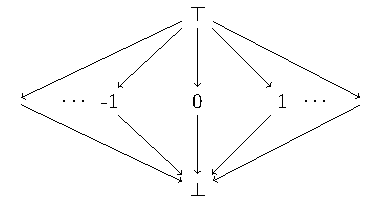
\includegraphics{constprop_lattice}
  \end{center}
  \vspace{-1em}
  \caption{Lattice commonly used to represent whether a variable is known to
           hold a constant value at a given program point.}
  \label{novillo:fig:lattice_constant_propagation}
\end{figure}

A key concept for data flow analysis is the representation of the property
space via \emph{partially ordered sets}. A partially ordered set $(L,
\sqsubseteq)$ is a set $L$ that is equipped with a reflexive, transitive, and
anti-symmetric relation $\sqsubseteq: L \times L \rightarrow \{true, false\}$.
Based on the relation an \emph{upper bound} for subsets of $L$ can be defined:
$l \in L$ is the upper bound for a subset $Y$ of $L$ if $\forall l' \in Y: l'
\sqsubseteq l$. Furthermore, $l \in L$ is the \emph{least upper bound} if it is
an upper bound and for any other upper bound $l_o$ of $Y$ : $l \sqsubseteq l_0$.
Lower bounds and greatest lower bounds are defined analogously.

A particularly interesting class of partially ordered sets are \emph{complete
lattices}, where all subsets have a least upper bound as well as a greatest
lower bound. These bounds are unique and are denoted by $\bigsqcup$ and
$\bigsqcap$. In the context of program analysis the former is often referred to
as the \emph{join operator}, while the latter is termed the \emph{meet
operator}. Complete lattices have two distinguished elements, the \emph{least
element} and the \emph{greatest element}, often denoted by $\bot$ and $\top$
respectively.

An \emph{ascending chain} is a totally ordered subset $\{l_1, \ldots, l_n \}$ of
a complete lattice, where for all $i, j \in \{1, \ldots, n\}, i < j: l_i
\sqsubseteq l_j$. A chain is said to \emph{stabilizes} if there exists an $i_0
\in \mathbb{N}$, where $\forall i \in \mathbb{N}, i > i_0: l_i = l_{i_0}$; $i_0$
is then called the \emph{length} of the chain.

Consider, for example, the lattice presented in
Figure~\ref{novillo:fig:lattice_constant_propagation} that is commonly used to
represent whether a given variable is known to hold a specific constant value at
a given program point at run-time. The analysis and the corresponding
optimization are often uniformly referred to as \emph{constant propagation}.
For this lattice, $\top$ indicates that no specific information on the
variable's value is known. The symbol $\bot$, on the other hand, indicates that
the analysis was not able to prove that the variable holds a constant value in
all cases. The other elements in the lattice denote that the variable is known
to hold the respective value. The $\sqsubseteq$ relation is represented by the
arrows in the figure. Clearly, all chains for this lattice are at most of length
three ($\bot \sqsubseteq c \sqsubseteq \top$, $c \in \mathbb{N}$).

%///////////////////////////////////////////////////////////////////////////////
\subsection{Program Representation}

\begin{figure}[b]
  \begin{center}
    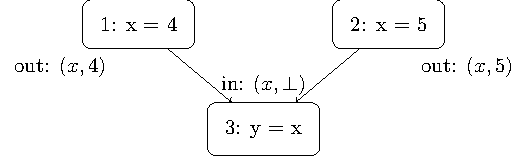
\includegraphics{contr_flow_graph}
  \end{center}
  \vspace{-1em}
  \caption{Combining data flow information using the join operator.}
  \label{novillo:fig:control_flow_graph}
\end{figure}

Individual functions of the input program are represented as separate flow
graphs of the form $G = (V,E)$, where the nodes represent operations, or
instructions, at a program point, and edges denote the possible flow of control
at run-time. The graph contains two distinguished nodes, the \emph{start} and
the \emph{exit} node, denoted by $s$ and $t$ respectively. These two nodes are
special in that the former is the only node that does not have any predecessor
and the latter is the only node without any successor.

During the analysis, data flow information is propagated from one node to
another adjacent node along the respective graph edge. Every node is associated
with data flow information using two sets, \emph{in} and \emph{out}. If the
target node has a single incoming edge only, the propagation corresponds to a
simple copy from the source node's \emph{out} set to the target node's \emph{in}
set. However, in the more general case of multiple incoming edges, we need to
combine the information from all those edges. This is accomplished by applying
the join or meet operator of the lattice that represents the property space. For
example, consider the lattice from
Figure~\ref{novillo:fig:lattice_constant_propagation} and the flow graph shown
in Figure~\ref{novillo:fig:control_flow_graph}. We can clearly say that, after
executing operation $1$ on the top left side, variable x holds the
constant value of $4$, as indicated by the \emph{out} annotation $(x, 4)$ below.
The same applies for operation $2$ on the right, with the slight difference that
the variable holds the value of $5$. Combining this information yields $4
\bigsqcup 5 = \bot$, i.e., x does not hold a constant value at program point 3.

In many cases it is helpful to reverse the flow graph to propagate information,
i.e., reverse the direction of the graph's edges. Analyses relying on this
reversed flow graph are termed \emph{backward analyses}, while those using the
regular flow graph are called \emph{forward analyses}. As shown before,
computing whether a variable holds a certain constant value is a forward
problem, while determining whether a computation is dead, i.e., not used, is a
typical backward problem.

We limit our discussion to \emph{intra-procedural} analyses that operate locally
on functions. Note, however, that data flow analysis can also be applied to
perform \emph{inter-procedural} analyses~\cite{novillo:bib:NNH99}.

%///////////////////////////////////////////////////////////////////////////////
\subsection{Transfer Functions}

\begin{table}[t]
  \begin{center}
    \begin{tabular}{lp{8mm}l}
      Operation                   & & Transfer Function                      \\ \hline
      x = $c$, $c \in \mathbb{N}$ & & $f_{x=c}(L) = L \setminus \{ (x, c') | (x, c') \in L \} \cup \{ (x, c) \}$ \\
      x = y                       & & $f_{x=y}(L) = L \setminus \{ (x, c') | (x, c') \in L \} \cup \{ (x, c) | (y,c) \in L\}$ \\
      x = $\ldots$                & & $f_{x=\ldots}(L) = L \setminus \{ (x, c') | (x, c') \in L \}$ \\
      $\ldots$                    & & $f_{\ldots}(L) = L$ \\ \hline
    \end{tabular}
  \end{center}
  \caption{A simplified set of transfer functions for constant propagation
           analysis.}
  \label{novillo:fig:transfer_functions}
\end{table}

Aside from the control flow, the effect of the program's operations
need to be accounted for during analysis. However, in contrast to the actual
execution, we are only interested in an abstract model of the operations'
effects with respect to the data flow information. Operations are thus mapped to
a set of abstract \emph{transfer functions} of the form $f_{op}: L \rightarrow
L$ that transform the information available from the \emph{in} set of the
respective flow graph nodes and store the result in the corresponding \emph{out}
set.

Continuing the example from above, a simple set of transfer functions can be
defined, as shown in Table~\ref{novillo:fig:transfer_functions}. Assignments to
variables invalidate the information that is available on that particular
variable. However, in the case of a copy operation or the assignment of a
constant value, new information is obtained.

%///////////////////////////////////////////////////////////////////////////////
\subsection{Solving Data Flow Problems}

Putting all those elements together, i.e., a complete lattice, a flow graph, and
a set of transfer functions, yields an instance of a monotone framework. Which,
in fact, describes a set of \emph{data flow equations} that need to be solved in
order to retrieve the analysis result. A very popular and intuitive way of
solving these equations is to compute the \emph{maximal fixed point} (MFP) using
an iterative work list algorithm. The work list contains operations that has
to be reevaluated by first combining the information form all their predecessors
in the flow graph, then applying their transfer function, and finally
propagating the obtained information to all successors by appending them to the
work list. The algorithm terminates when the data flow information stabilizes
and the work list becomes empty~\cite{novillo:bib:NNH99}.

It is obvious that a single flow edge can be appended several times to the
work list in the course of the analysis. It may even happen that an infinite
feedback loop prevents the algorithm from terminating. We are thus interested in
bounding the number a given edge is processed. Recalling the definition of
chains from Section~\ref{novillo:sec:property_space}, the \emph{height} of a
lattice is defined by the length of its longest chain. We can ensure termination
for lattices fulfilling the \emph{ascending chain condition}, which ensures that
the lattice has finite height. Given a lattice with finite height $h$ and a flow
graph $G=(V, E)$ it is easy to see that the MFP solution can be computed in
$O(|E| \cdot h)$ time, or, due to the fact that $|E| \leq |V|^2$, in $O(|V|^2
\cdot h)$. Note that the height of the lattice often depends on properties of
the input program, which might ultimately yield bounds worse than cubic in the
number of graph nodes. \obacht{TODO:}{Talk about Memory consumption?}

For reducible flow graphs the order in which operations are processed by the
work list algorithm can be
optimized~\cite{novillo:bib:HU73,novillo:bib:KU76,novillo:bib:NNH99}, allowing
to derive tighter complexity bounds. However, relying on reducibility is
problematic, because flow graphs are often \emph{not} reducible even for proper
structured languages, e.g., reversed flow graphs of backward problems can be,
and in fact almost always are, irreducible even for programs with reducible flow
graphs. Furthermore, experiments have shown that the tighter bounds not
necessarily lead to improved compilation times~\cite{novillo:bib:CTK06}.

Apart from computing a fixed point, data flow equations can also be solved using
a more powerful approach called the \emph{meet over all paths} (MOP) solution.
Even though more powerful, computing the MOP solution is often harder or even
undecidable~\cite{novillo:bib:NNH99}. Consequently, the MFP solution is
preferred in practice.

%%%%%%%%%%%%%%%%%%%%%%%%%%%%%%%%%%%%%%%%%%%%%%%%%%%%%%%%%%%%%%%%%%%%%%%%%%%%%%%%
\section{Propagation Engine}
\label{novillo:sec:prop-engine} \obacht{Rename?}{Propagation under SSA Form}

SSA form allows to solve a large class of data flow problems more efficiently
than the standard fixed point solution presented previously. The basic idea is
to directly propagate information computed at the unique definition of a
variable to all its uses. Intermediate program points on regular control flow
paths from the definition to those uses are skipped, reducing memory consumption
and compilation time.

%///////////////////////////////////////////////////////////////////////////////
\subsection{Program Representation}

Programs in SSA form exhibit, aside from the regular operations of the original
program, special operations called $\phi$-operations, which are placed at join
points of the original CFG -- see Part~\ref{part:vanilla_ssa} of this book for
more information. In the following, we assume that possible many
$\phi$-operations are associated with the corresponding CFG nodes at those
join points.

\obacht{Reference for SSA graphs}{Point directly to a chapter in the book?}
Data flow analysis under SSA form relies on a specialized program
representation based on \emph{SSA graphs}~\cite{novillo:bib:CFRWZ91}, which
allows to simplify the propagation of data flow information. The nodes of an
SSA graph correspond to the operations of the program. In particular the
program's $\phi$-operations are represented by dedicated nodes in the SSA graph.
The edges of the graph connect the unique definition of a variable with all its
uses, i.e., an edge represents a true data dependence among two nodes.

An important property of SSA graphs is that they also capture, besides the data
dependencies, the \emph{relevant} join points of the program's CFG. A join point
is relevant for the analysis, whenever the value of two or more definitions may
reach a use by passing through that join. Due to the properties of SSA form, it
is ensured that a $\phi$-operation is placed at the join point and that the use
has been properly updated to refer to the respective $\phi$-operation. Other
join points can safely be ignored, because uses are guaranteed to receive the
same value on all paths due to the dominance property.

\begin{figure}[t]
  \begin{center}
    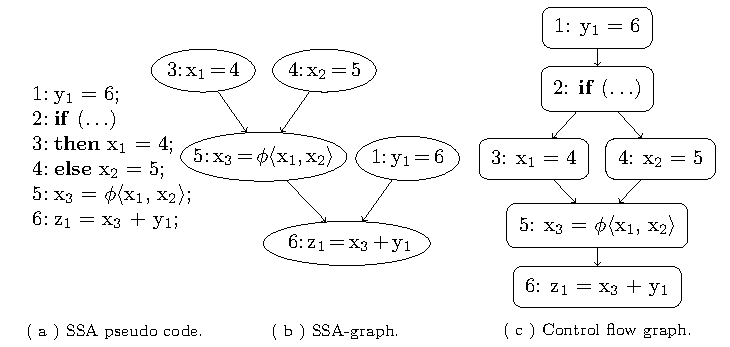
\includegraphics{ssa_graph}
  \end{center}
  \vspace{-2em}
  \caption{Example program and its SSA graph.}
  \label{novillo:fig:ssa_graph}
\end{figure}

Consider for example, the code excerpt shown in
Figure~\ref{novillo:fig:ssa_graph}, along with the corresponding SSA graph and
CFG. Assume we are interested in propagating information from the assignment of
variable y$_1$ at the beginning of the code excerpt down to its unique use at
the end. Using the traditional CFG representation this requires the propagation
through several intermediate program points. These program points are concerned
with computations of the variables x$_1$  through x$_3$ only and are thus
irrelevant for the computation at hand. The SSA graph representation, on the
other hand, allows to propagate the desired information directly without any
intermediate steps. At the same time, we also find that the control flow join
following the \textbf{if} is properly represented by the $\phi$-operation
defining the variable x$_3$ in the SSA graph.

Even though the SSA graph captures data dependencies and the relevant join
points in the CFG, it lacks information on other
\emph{control dependencies}. However, analysis results can often be improved
significantly by considering the additional information that is available from
the control dependencies in the program's CFG. As an example consider once more
the code excerpt shown in Figure~\ref{novillo:fig:ssa_graph}. Assume that the
condition associated with the \textbf{if} operation is known to be false for all
possible program executions. Consequently, the $\phi$-operation will select the
value of x$_2$ in all cases, which is known to be of constant value $5$.
However, due to the shortcomings of the SSA graph this information cannot be
derived. It is thus important to use both graphs during data flow analysis
in order to obtain the best possible results.

%///////////////////////////////////////////////////////////////////////////////
\subsection{Sparse Data Flow Propagation}

\begin{algorithm}[t!]
  \begin{enumerate}
    \item Initially, every edge in the CFG is marked not executable and the
          \emph{FlowWorkList} is seeded with the outgoing edges of the flow
          graph's \emph{start} node.  The \emph{SSAWorkList} is empty.
    \item \label{novillo:alg:propagation:loop} Remove the top element of either
          of the two work lists.
    \item \label{novillo:alg:propagation:flowedge} If the element is a flow edge
          that is marked to be executable, do nothing, \\ otherwise proceed as
          follows:
          \begin{itemize}
            \item Mark the edge as executable.
            \item Visit every $\phi$-operation associated with the edge's target
                  node.
            \item When the target node was reached the first time via the
                  \emph{FlowWorkList} visit its operation.
            \item When the target node has a single outgoing non-executable edge
                  append that edge to the \emph{FlowWorkList}.
          \end{itemize}
    \item \label{novillo:alg:propagation:ssaedge} If the element is an edge from
          the SSA graph, process the target operation as follows:
          \begin{enumerate}
            \item[a.] When the target operation is a $\phi$-operation visit that
                      $\phi$-operation.
            \item[b.] \label{novillo:alg:propagation:ssaedge:regular} For
                      regular target operations, examine the corresponding
                      executable flag of the incoming edges of its corresponding
                      flow graph node. If any of those edges is marked
                      executable visit the operation, otherwise do nothing.
          \end{enumerate}
    \item Continue with step \ref{novillo:alg:propagation:loop} until both work
          lists become empty.
    \vspace{-1em}
  \end{enumerate}

  \caption{Sparse Data Flow Propagation}
  \label{novillo:alg:propagation}
\end{algorithm}

Similar to monotone frameworks for traditional data flow analysis, frameworks
for \emph{sparse data flow propagation} under SSA form can be defined. As
before, such a framework consist of: (1) a complete lattice, (2) a set of
transfer functions, (3) a flow graph, and additionally (4) an SSA graph. We
again seek a maximal fixed point solution (MFP) using an iterative work list
algorithm. However, in contrast to the algorithm described before, data flow
information is not propagated along the edges of the flow graph but along the
edges of the SSA graph. For regular uses the propagation is straightforward due
to the fact that every use receives its value from a unique definition. Special
care has to be taken for $\phi$-operations, which select a value among their
operands depending on the incoming flow edges. The data flow information of the
incoming operands has to be combined using the meet operator of the lattice.
Furthermore, the flow graph is used in order to track which operations are not
reachable under any program execution and thus can be safely ignored during the
computation of the fixed point solution.

The algorithm processes two work lists, the \emph{FlowWorkList} containing edges
of the flow graph and the \emph{SSAWorkList}, which consists of edges from the
SSA graph. It proceeds by removing the top element of either of those lists and
processing the respective edge as indicated by
Algorithm~\ref{novillo:alg:propagation}. Throughout the algorithm operations of
the program may be visited in order to update the work lists and propagate
information as shown by Algorithm~\ref{novillo:alg:visit}. We will highlight
the most relevant parts of the algorithms in the following paragraphs and
explain some important aspects of their interaction.

\begin{algorithm}[t!]
  \begin{enumerate}
    \item Compute the operation's data flow information:
    \begin{enumerate}
      \item[a.] \label{novillo:alg:visit:phi} If the operation is a
                $\phi$-operation, combine the data flow information from all its
                operands where the corresponding flow edge is marked executable.
      \item[b.] \label{novillo:alg:visit:branch} In the case of conditional
                branches, update the operation's data flow information. Determine
                which of the outgoing flow edges are reachable from the
                corresponding flow graph node by examining the branch's
                condition(s) and append the respective non-executable edges to
                the \emph{FlowWorkList}.
      \item[c.] \label{novillo:alg:visit:regular} For regular operations, update
                the corresponding data flow information by applying its transfer
                function.
    \end{enumerate}
    \item Whenever the data flow information changes append all outgoing edges
          of the corresponding SSA graph node to the \emph{SSAWorkList}.
    \vspace{-1em}
  \end{enumerate}
  \caption{Visiting an Operation}
  \label{novillo:alg:visit}
\end{algorithm}

In step~\ref{novillo:alg:propagation:flowedge} of the main algorithm, flow edges
are processed that were encountered to be executable for the first time in the
course of the analysis. Whenever such a flow edge is processed, all
$\phi$-operations of its target node need to be reevaluated due to the fact that
Algorithm~\ref{novillo:alg:visit}a discarded the respective operands of the
$\phi$-operations so far -- because the flow edge was not yet marked executable.
Similarly, the operation of the target node has to be evaluated when the target
node is encountered to be executable for the first time, i.e., the currently
processed edge is the first of its incoming edges that is marked executable.
Note that this is only required the \emph{first} time the node is
encountered to be executable, due to the processing of operations in
Step~\ref{novillo:alg:propagation:ssaedge}b, which thereafter triggers the
reevaluation automatically when necessary.

Regular operations as well as $\phi$-operations are visited by
Algorithm~\ref{novillo:alg:visit} whenever the corresponding flow graph node has
become executable or when the data flow information of one of its predecessors
in the SSA graph changed. $\phi$-operations combine the information from
multiple flow paths using the usual meet operator, but only considering those
operands where the associated edge is marked executable. Conditional branches
are handled by examining its conditions based on the data flow information
computed so far. Depending on whether those conditions are satisfiable or not,
flow edges are appended to the \emph{FlowWorkList} in order to ensure that all
reachable operations are considered during the analysis. Finally, all regular
operations are processed by applying the relevant transfer function and possibly
propagating the updated information to all uses by appending the respective
SSA graph edges to the \emph{SSAWorkList}.

\begin{figure}[t!]
  \begin{center}
    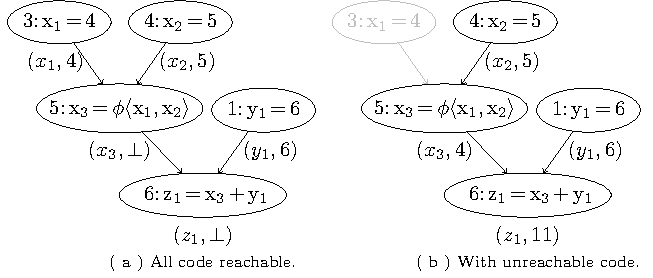
\includegraphics{ssa_propagation}
    \subfigure{\label{novillo:fig:ssa_propagation:a}}
    \subfigure{\label{novillo:fig:ssa_propagation:b}}
  \end{center}
  \vspace{-2em}
  \caption{Sparse data flow propagation using SSA graphs.}
  \label{novillo:fig:ssa_propagation}
\end{figure}

\obacht{Example:}{Do we need a more detailed description of the work lists?}
As an example, consider the program shown in Figure~\ref{novillo:fig:ssa_graph}
and the constant propagation problem. First,
assume that the condition of the \textbf{if} can not be statically evaluated.
Consequently, all flow edges in the program will eventually be marked
executable. This will trigger the evaluation of the constant assignments to
the variables x$_1$,  x$_2$, and y$_1$. The transfer functions immediately yield
that the variables are all constant holding the value $4$, $5$, and $6$
respectively. This new information will trigger the reevaluation of the
$\phi$-operation of variable x$_3$. As both of its operands are reachable the
combined information yields $3 \bigsqcup 5 = \bot$. Finally, also the assignment
to variable z$_1$ is reevaluated, but the analysis shows that its value is not a
constant as depicted by Figure~\ref{novillo:fig:ssa_propagation:a}. If, however,
the condition of the \textbf{if} is known to be false for all possible program
executions a more precise result can be computed, as shown in
Figure~\ref{novillo:fig:ssa_propagation:b}. Neither the flow edge leading to the
assignment of variable x$_1$ is marked executable nor its outgoing edge leading
to the $\phi$-operation of variable x$_3$. Consequently, the reevaluation of
the $\phi$-operation only considers the data flow information of its second
operand x$_2$, which is known to be constant. This finally enables to analysis
to show that the assignment to variable z$_1$ is in fact constant as well.

\obacht{Complexity results}{\begin{itemize}
                              \item Relate to bounds of traditional data flow
                                    analysis,
                              \item Do we have any numbers that propagation is
                                    faster under SSA form?
                              \item Memory consumption: Point out that we can
                                    keep data flow information with every
                                    definition.
                            \end{itemize}
}
During the course of the propagation algorithm every edge of the SSA graph is
processed at least once, whenever the operation corresponding to its definition
is found to be executable. Afterward, an edge can be revisited several times
depending on the height $h$ of the lattice representing the analysis' property
space. Reachable edges of the flow graph, on the other hand, are processed at
most once. This leads to an upper bound in execution time of $O(|E_{SSA}| \cdot
h + |E_{FG}|)$, where $E_{SSA}$ and $E_{FG}$ represent the edges of the
SSA graph and the flow graph respectively -- see~\cite{bib:wegman.ea-91}.

%///////////////////////////////////////////////////////////////////////////////
\subsection{Limitations}

Unfortunately, the presented approach also has its drawbacks in terms of
general applicability. The problem arises from two sources: (1) the exclusive
propagation of information between data-dependent operations and (2) the
semantics and placement of $\phi$ operations. The former issue prevents the
modeling of data flow problems that propagate information to program points that
are not directly related to either a definition or a use of a variable, while
the latter prevents the modeling of backward problems.

Consider, for example, the well known problem of available
expressions~\cite{novillo:bib:NNH99} that often occurs in the context of
redundancy elimination. An expression is available at a given program point when
the expression is computed, and not modified thereafter, on all paths leading to
the program point. In particular, this might include program points that are
independent from the expression and its operands, i.e., neither defines nor uses
any of its operands. However, the SSA graph does not cover those program points
as it propagates information directly from definitions to uses without any
intermediate steps.

Furthermore, data flow analysis using SSA graphs is limited to forward problems.
Due to the structure of the SSA graph it is not possible to simply reverse the
edges in the graph as it is done with flow graphs. For one, this would
invalidate the nice property of having a single source for incoming edges of a
given variable, as variables typically have more than one use. In addition,
$\phi$-operations are placed at join points with respect to the \emph{forward}
control flow and thus do not capture join points in the reversed flow graph.
SSA graphs are consequently not suited to model backward problems.

Even though the presented approach has its restrictions, it lead the way to the
development of advanced sparse data flow techniques, such as the \emph{sparse
evaluation graph} by Choi~et.al.~\cite{novillo:bib:CCF91} or the \emph{compact
evaluation graph}~\cite{novillo:bib:R02}. Those graphs can be computed for both,
backward and forward problems, and allow to propagate information to program
points independent of definitions and uses of certain variables. Nevertheless,
data flow analysis based on SSA graphs is still a useful and effective solution
for many interesting problems, as will be shown in the following sections. We
will also highlight the fact that SSA form is still helpful in solving
traditional backward problems such as dead code elimination.

%%%%%%%%%%%%%%%%%%%%%%%%%%%%%%%%%%%%%%%%%%%%%%%%%%%%%%%%%%%%%%%%%%%%%%%%%%%%%%%%
\section{Copy Propagation}
\label{novillo:sec:copy-prop}

Copy propagation in SSA form is, in principle, very simple.  Given the
assignment \linebreak $x = y$, all we need to do is traverse all the immediate
uses of $x$ and replace them with $y$, thereby effectively eliminating the
original copy operation. However, such an approach will not be able to propagate
copies past $\phi$-operations, particularly those in loops. A more powerful
approach is to split copy propagation into two phases. First, data flow analysis
is performed in order to find copy-related variables throughout the program.
Followed by a rewrite phase that eliminates spurious copies and renames
variables.

\begin{figure}[b!]
  \begin{center}
    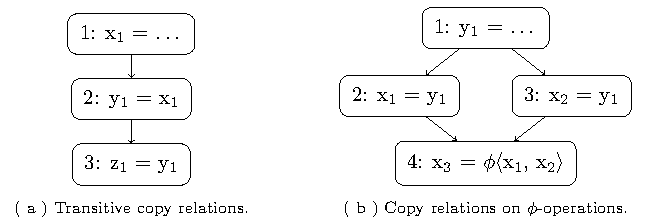
\includegraphics{copy_propagation}
    \subfigure{\label{novillo:fig:copy_propagation:a}}
    \subfigure{\label{novillo:fig:copy_propagation:b}}
  \end{center}
  \vspace{-1em}
  \caption{Analysis of copy-related variables.}
  \label{novillo:fig:copy_propagation}
\end{figure}

The data flow problem for copy propagation can be described as the problem of
propagating the \textit{copy of} value of variables.  Given a sequence of
copies as shown in Figure~\ref{novillo:fig:copy_propagation:a}. We say that
y$_1$ is a \textit{copy of} x$_1$ and z$_1$ is a \textit{copy of} y$_1$.  The
problem with this representation is that there is no apparent link from z$_1$ to
x$_1$.  In order to handle transitive copy relations, all transfer functions
operate on copy-of values instead of the direct source of the copy.  If a
variable is not found to be a copy of anything else, its copy-of value is the
variable itself. For the example above, this yields that both, y$_1$ and z$_1$,
are copies of x$_1$, which in turn is a copy of itself. The lattice of this data
flow problem is thus similar to the lattice shown previously for constant
propagation. However, the lattice elements correspond to variables of the
program instead of integer numbers and the least element of the lattice
represents the fact that the variable is a copy of itself.

Similarly, we would like to obtain the result that x$_3$ is a copy of y$_1$ for
the example depicted in Figure~\ref{novillo:fig:copy_propagation:b}. This is
accomplished by choosing the meet operator such that a copy relation is
propagated whenever the copy-of values of all the $\phi$-operation's operands
match. So, when visiting the $\phi$-operation for x$_3$, the propagator finds
that x$_1$ and x$_2$ are both copies of y$_1$, which allows to propagate the
desired result that x$_3$ is a copy of y$_1$.

The following example shows a more complex situation where copy relations are
obfuscated by loops -- see Figure~\ref{novillo:fig:copy_propagation_loop}.  Note
that the actual visiting order depends on the shape of the CFG and immediate
uses, the ordering used here is meant for illustration only. Processing starts
at the operation labeled $1$, with both work lists empty and the data flow
information $\top$ associated with all variables:

\begin{figure}[b!]
  \begin{center}
    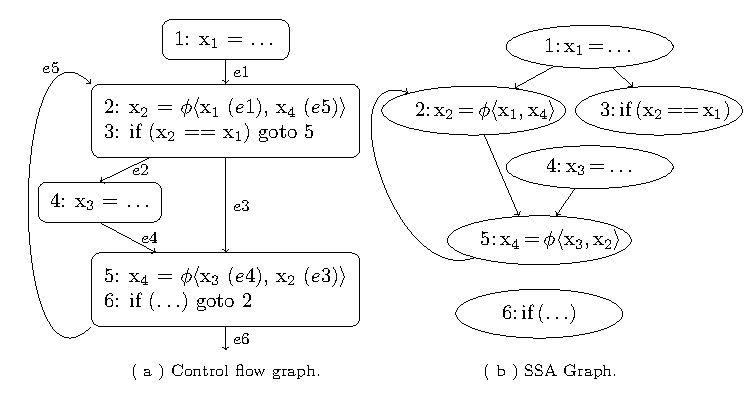
\includegraphics{copy_propagation_loop}
  \end{center}
  \vspace{-1em}
  \caption{$\phi$-operations in loops often obfuscate copy relations.}
  \label{novillo:fig:copy_propagation_loop}
\end{figure}

\begin{enumerate}
\item Assuming that the value assigned to variable x$_1$ is not a copy, the data
      flow information for this variable is lowered to $\bot$, the SSA edges
      leading to operations $2$ and $3$ are appended to the \emph{SSAWorkList},
      and the flow graph edge $e1$ is appended to the \emph{FlowWorkList}.
\item \label{novillo:copy_prop:ex:x_2} Processing the flow edge from the
      work list causes the edge to be marked executable and the operations
      labeled $2$ and $3$ to be visited. Since, edge $e5$ is not yet known to be
      executable the processing of the $\phi$-operation yields a copy relation
      between x$_2$ and x$_1$. This information is utilized in order to
      determine which outgoing flow graph edges are executable for the
      conditional branch. Examining the condition shows that only edge $e3$ is
      reachable and thus needs to be added to the work list.
\item Flow edge $e3$ is processed next and marked executable for the first time.
      Furthermore, the $\phi$-operation labeled $5$ is visited. Due to the fact
      that edge $e4$ is not known the be executable, this allows to discover a
      copy relation between x$_4$ and x$_1$ (via x$_2$). The condition of the
      branch labeled $6$ cannot be analyzed and thus causes its outgoing flow
      edges $e5$ and $e6$ to be added to the work list.
\item Now, flow edge $e5$ is processed and marked executable. Since the target
      operations are already known to be executable, only the $phi$-operation is
      revisited. However, variables x$_1$ and x$_4$ have the same copy-of value
      x$_1$, which is identical to the previous result computed in
      Step~\ref{novillo:copy_prop:ex:x_2}. Thus, neither of the two work lists
      is modified.
\item Assuming that the flow edge $e6$ leads to the exit node of the flow graph
      the algorithm stops after processing the edge without modifications to
      the data flow information computed so far.
\end{enumerate}

The straightforward implementation of copy propagation, would have needed
multiple passes to discover that x$_4$ is a copy of x$_1$.  But the iterative
nature of the propagation along with the ability to discover non-executable
code allows to handle even obfuscated copy relations. Moreover, this kind of
propagation will only reevaluate the subset of operations affected by newly
computed data flow information instead of the complete flow graph once the set
of executable operations has been discovered.

\section{Value Range Propagation}
\label{novillo:sec:vrp}

This transformation is similar to constant propagation, which served as a
running example throughout this chapter. But instead of propagating single
constant values, contiguous value ranges for variables are propagated. For
instance, the code in Figure \ref{novillo:fig:vrp-1} is extracted from a
typical expansion of bound checking code in languages like Java. Notice how the
bounds check at line $12$ is not really necessary as variable $i$
is guaranteed to take values in the range [$0$, a-\textgreater len - 1].

\begin{figure}
  \begin{center}
    \begin{tabular}{c}
      \begin{lstlisting}
struct array
{
  const int len;
  int *data;
};

void
doit(array *a)
{
  for (int i = 0; i < a->len; ++i)
    {
      if (i < 0 || (i) >= (a->len))
        throw 5;
      call (a->data[i]);
    }
}
      \end{lstlisting}
    \end{tabular}
  \end{center}
  \caption{Useless array-bound checking code.}
  \label{novillo:fig:vrp-1}
\end{figure}

Value range propagation works in two main phases:

\begin{enumerate}
\item  Range Assertions.  Some expressions like predicates in
       conditional jumps, pointer dereferences or taking the
       absolute value of a variable imply something about the
       range of values that their result may take.  For
       instance, the expression \lcode{if (a_5 > 10) ...}
       implies that every use of a$_5$ inside the if will be
       guaranteed to use values in the range [$11$, +INF].

       For every expression in this category, the compiler
       generates a new expression code (\lcode{ASSERT_EXPR})
       that describes the guaranteed range of values taken by
       the associated name.

\item  Range Propagation.  Once \lcode{ASSERT_EXPR} instructions
       have been inserted, the SSA propagation engine is used to
       evaluate the program.  After propagation, every SSA name
       created by the program will have a range of values
       associated with it.  Those ranges are then used to
       eliminate conditional jumps made superfluous by the new
       range information.
\end{enumerate}

\subsection{Inserting range assertions}

Certain expressions found in the code give us information about
the range of values that may be taken by the operands involved in
the expression.  For instance, consider the code fragment in
Figure \ref{novillo:fig:assert-expr-before}.

\begin{figure*}
  \centering
  \begin{tabular}{cc}
      \begin{minipage}[b]{0.45\textwidth}
        \begin{lstlisting}[showlines=true]

$p_4$ = $p_3$ + 1;

if ($p_4$ == 0)
  return 0;

$x_{10}$ = *$p_4$;

if ($p_4$ == 0)
  return 0;

if ($a_5$ == 10)
  return $a_5$ + $x_{10}$;

return $a_5$ - $x_{10}$;

        \end{lstlisting}
        \subfigure[Before inserting assertions.]{
          \hspace{0.8\textwidth}
          \label{novillo:fig:assert-expr-before}
        }
      \end{minipage}
      &
      \begin{minipage}[b]{0.53\textwidth}
        \begin{lstlisting}
$p_4$ = $p_3$ + 1;

if ($p_4$ == 0)
  return 0;

$x_{10}$ = *$p_4$;
$p_5$ = ASSERT_EXPR<$p_4$, $p_4$ != 0>;

if ($p_5$ == 0)
  return 0;

if ($a_5$ == 10)
  $a_6$ = ASSERT_EXPR<$a_5$, $a_5$ == 10>;
  return $a_6$ + $x_{10}$;

return $a_5$ - $x_{10}$;
      \end{lstlisting}
        \subfigure[After inserting assertions.]{
          \hspace{0.8\textwidth}
          \label{novillo:fig:assert-expr-after}
        }
      \end{minipage}

  \end{tabular}
  \caption{Preparing the program for Value Range Propagation.}
\end{figure*}

Since pointer p$_4$ is dereferenced at line $6$, we know that the
NULL test at line $8$ must always fail.  Similarly, the use of
a$_5$ at line $12$ is guaranteed to always use the constant value
$10$.  However, we cannot guarantee that \textbf{all} uses of
p$_4$ and a$_5$ will always have a known value.  For instance,
we have no way of knowing at compile time whether the NULL test
for p$_4$ at line $3$ will succeed or not.  Similarly, the use of
a$_5$ at line $14$ does not use a known value.

The technique used by VRP to overcome this problem is to create
new SSA names to which we can pin the range information that we
want to propagate.  The compiler generates a new expression called
\lcode{ASSERT_EXPR} that captures this information and stores it
into a new SSA name.  When the compiler finds an expression that
contains interesting range information for name $N_i$, it
builds a predicate P describing that range and generates
the assignment \lcode{N_j = ASSERT_EXPR <N_i, P>}.  This
expression means that variable $N_j$ has the same value as $N_i$
\textbf{and} that value is guaranteed to make predicate P
evaluate to \textit{true}.

Therefore, for the code in Figure
\ref{novillo:fig:assert-expr-before}, the compiler inserts the
assertions found in Figure \ref{novillo:fig:assert-expr-after}.
The pointer dereference in line $6$ produces the assertion
p$_5$ = \lcode{ASSERT_EXPR <}p$_4$, p$_4$ != $0$\lcode{>}.  With
this conversion, all uses of p$_5$ are guaranteed to be uses of a
non-NULL pointer.  Similarly, uses of a$_6$ are guaranteed to use
the constant value $10$.

\subsection{Incremental updates of the SSA form}

Since range assertion expressions are inserted once the program
is in SSA form, it must be updated before ranges are propagated.
Each expression $N_i$ = \lcode{ASSERT_EXPR <}$N_j$, P\lcode{>}
creates a mapping from the existing name $N_j$ to the new name
$N_i$.

As assertions are inserted in the IL, a replacement mapping is
built.  In the example code of Figure
\ref{novillo:fig:assert-expr-after}, the compiler will build two
mappings, namely p$_5 \rightarrow$ p$_4$ and a$_6 \rightarrow$
a$_5$.  Once all the assertions have been inserted, the SSA form
can be incrementally updated by applying all the name mappings.

The mechanics of the updating process are a little more
elaborate than this, but in essence all it does is search and
replace inside the sub-regions of the CFG affected by the
existing names and their replacements.

\subsection{Propagating ranges}

\begin{figure}
    \centering
    \parbox{2in}{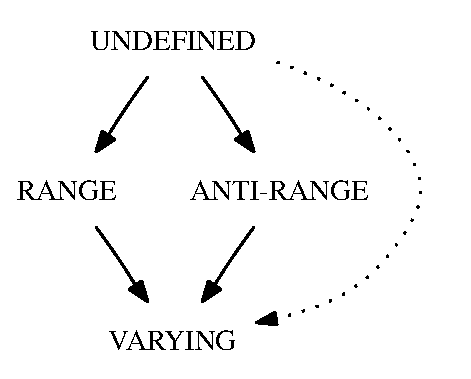
\includegraphics[height=2in]{vrp-4}}
    \caption{Lattice values used for range propagation.}
    \label{novillo:fig:vrp-lattice}
\end{figure}

The range propagation lattice has 4 values as shown in Figure
\ref{novillo:fig:vrp-lattice}.  As is the case with other
propagation problems, the only valid transitions are those that
move downward in the lattice.  If we were to allow transitions in
different directions, we would risk infinite loops during
propagation.

Lattice values \textsc{RANGE} and \textsc{ANTI-RANGE} are exactly
the same in terms of propagation, they both represent known
range values for the associated SSA names.  The key difference is
in the semantics of the actual value when evaluating expressions.

Two types of statements are considered interesting by the
propagator:

\begin{enumerate}
\item	Assignments of the form $N_i$ = EXPR, where EXPR is of
	an integral or pointer type.  The expression is evaluated
	and if it results in a useful range, its value is
	associated to $N_i$.

	Naturally, the more common sources of useful range
	information are \lcode{ASSERT_EXPR}s, but other
	expressions may also provide useful ranges.  For
	instance, if EXPR is $42$, then we can set the range of
	$N_i$ to $[42, 42]$.  Similarly, expressions involving
	names with known ranges may yield useful information.

\item	Conditional branches are also evaluated.  If the
	controlling predicate includes names with known ranges,
	only the taken edges are added to the CFG work list.
\end{enumerate}

Evaluation of $\phi$ nodes uses the usual shortcut of ignoring
arguments coming through non-executable edges.  Given two
arguments with ranges VR0 and VR1:

\begin{enumerate}
\item	If VR0 and VR1 have an empty intersection the resulting
	range is set to VARYING.

\item	Otherwise, the resulting range is VR0 $\bigcup$ VR1.
\end{enumerate}

Propagation continues while names change from one state to the
other.  Once all the basic blocks have been simulated and no
state transitions occur, simulation stops.

%%%%%%%%%%%%%%%%%%%%%%%%%%%%%%%%%%%%%%%%%%%%%%%%%%%%%%%%%%%%%%%%%%%%%%%%%%%%%%%%
\section{Dead Code elimination}
\label{novillo:sec:dead_code_elimination}

%%%%%%%%%%%%%%%%%%%%%%%%%%%%%%%%%%%%%%%%%%%%%%%%%%%%%%%%%%%%%%%%%%%%%%%%%%%%%%%%
\section{Conclusion}
\label{novillo:sec:conclusion}

